\subsection{Eclipse plugin}
Gradle mette a disposizione anche dei plugin esclusivi per gli IDE (Integrated development environment). Considereremo il caso dell'IDE Eclipse a cui sono associati 2 plugin:
\begin{itemize}
    \item \texttt{eclipse-wtp} (Eclipse Web Tools Platform Project)
    \item \texttt{eclipse}
\end{itemize}
Questi plugin aggiungono alcuni tasks molto importanti per progetti sviluppati su questo IDE (è possibile trovare tutti i task nella documentazione relativa: \textit{\href{https://docs.gradle.org/current/userguide/eclipse\_plugin.html\#sec:eclipse\_tasks}{docs.gradle.org/current/userguide/eclipse\_plugin.html}}). Creiamo quindi un nuovo progetto java eseguendo il task init:
\begin{verbatim}
    $ gradle init --type java-application\end{verbatim}
Andiamo a modificare il build.gradle aggiungendo il plugin \texttt{eclipse}:
 \begin{lstlisting}[frame=single]
plugins {
    id 'eclipse'
} \end{lstlisting}
Se andiamo ora a eseguire la build tasks per vedere quali tasks il nostro progetto Gradle ha a disposizione vedremo che nell'output ci sarà una sezione definita \textbf{IDE tasks}:
\begin{verbatim}
IDE tasks
---------
cleanEclipse - Cleans all Eclipse files.
eclipse - Generates all Eclipse files. \end{verbatim}
Possiamo ora quindi eseguire la build \texttt{eclipse} per generare tutti i file necessari per un progetto eclipse:
\begin{verbatim}
    $ ./gradlew eclipse\end{verbatim}
La build genererà 2 files che sono: \texttt{.classpath} e \texttt{.project}, e 1 directory che è \texttt{.settings}, questi 3 elementi servono all'IDE per identificare e generare i dati di un progetto. A questo punto possiamo aprire eclipse e importare il progetto che abbiamo appena creato:
\begin{figure}[H]
    \centering
    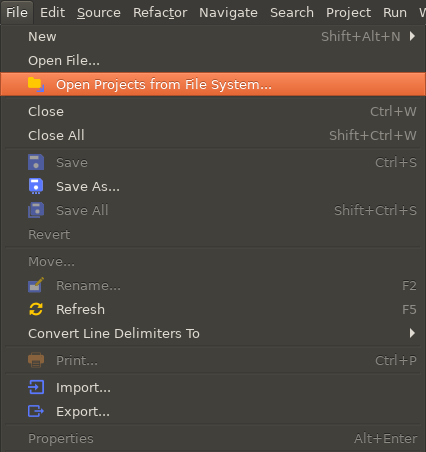
\includegraphics[width=0.4\linewidth]{3DependencyManagement/eclipsePlugin/openProject.png}
\end{figure}
Si aprirà una finestra in cui ci sarà un campo \texttt{import source} dove dovremo indicare il percorso specifico del progetto. Il risultato sarà un progetto contenente questo:
\begin{figure}[H]
    \centering
    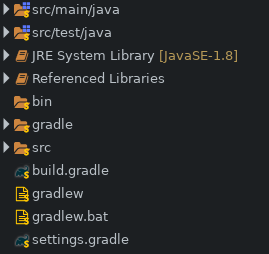
\includegraphics[width=0.4\linewidth, height=5cm]{3DependencyManagement/eclipsePlugin/resultProject.png}
\end{figure}
Tutto questo procedimento è possibile farlo direttamente da Eclipse, infatti installando il plugin chiamato \texttt{Buildship Gradle Integration 2.0} è possibile creare un nuovo progetto Gradle. Per farlo basterà cliccare su \texttt{File -> New -> Other...} che farà apparire una finestra di selezione wizard di progetto:
\begin{figure}[H]
\begin{subfigure}{0.5\textwidth}
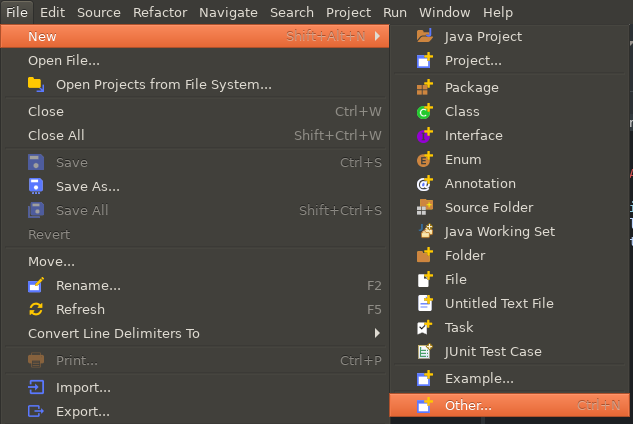
\includegraphics[width=0.9\linewidth, height=7cm]{3DependencyManagement/eclipsePlugin/newProject.png}
\end{subfigure}
\begin{subfigure}{0.5\textwidth}
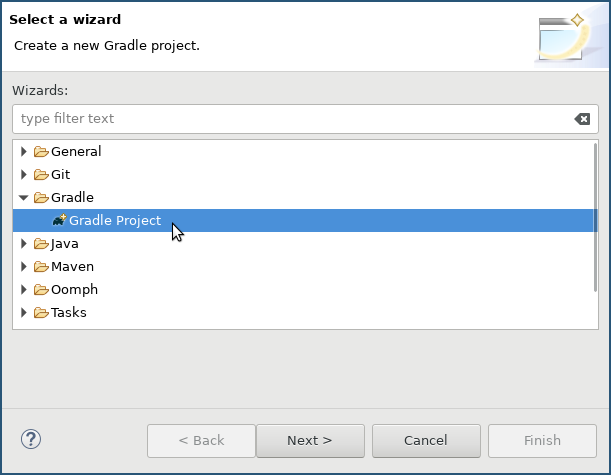
\includegraphics[width=0.9\linewidth, height=7cm]{3DependencyManagement/eclipsePlugin/wizardGradle.png}
\end{subfigure}
\end{figure}
Dopo aver indicato la posizione e il nome del progetto, sarà richiesto se usare il wrapper Gradle o di specificare la posizione in locale di Gradle. Ci sarà poi un riassunto generale e cliccando su finish il progetto verrà creato. Notiamo che non ci sono differenze tra la versione del progetto generata con questa modalità o con il procedimento da terminale, infatti eclipse automatizzerà solo i procedimenti di creazione ma non il modo di creazione. Il plugin di Gradle per eclipse mette a disposizione anche una versione grafica per eseguire le build includendo 2 finestre:
\begin{itemize}
    \item Gradle Tasks, che restituisce la lista dei tasks relativi al progetto selezionato
    \item Gradle Executions, che è in poche parole l'output della build eseguita in formato non terminale
\end{itemize}
Per poterle aggiungere dobbiamo andare su \texttt{Window -> Show View -> Other...} e poi selezionare le due view di Gradle:
\begin{figure}[H]
\begin{subfigure}{0.6\textwidth}
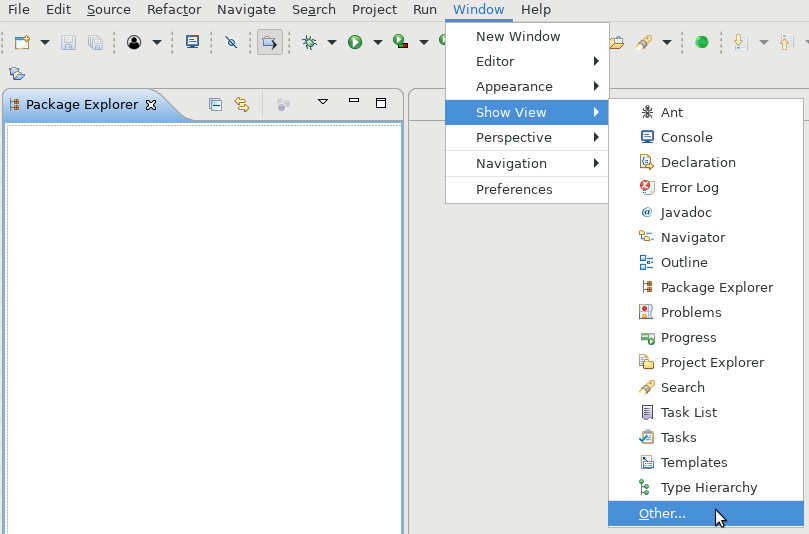
\includegraphics[width=1.0\linewidth, height=7cm]{3DependencyManagement/eclipsePlugin/openShowView.png}
\end{subfigure}
\begin{subfigure}{0.6\textwidth}
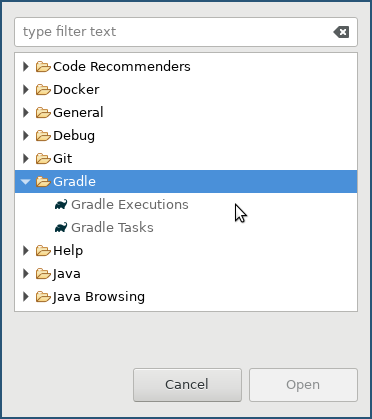
\includegraphics[width=0.6\linewidth, height=7cm]{3DependencyManagement/eclipsePlugin/gradlePluginFeature.png}
\end{subfigure}
\end{figure}
Usando questa view possiamo eseguire direttamente i task che vogliamo, per esempio se volessimo eseguire il task \texttt{test} basterà cliccare con il destro e poi su \texttt{Run Gradle Tasks}:
\begin{figure}[H]
    \centering
    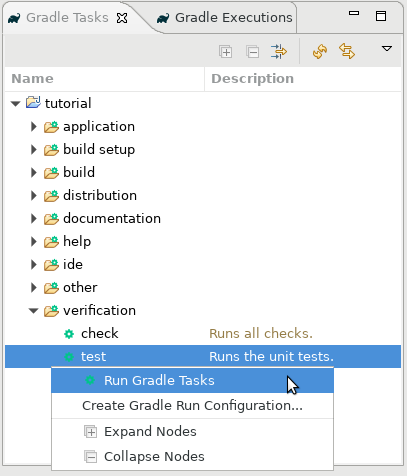
\includegraphics[width=0.4\linewidth]{3DependencyManagement/eclipsePlugin/runTestTask.png}
\end{figure}
Noteremo che sia la view  \texttt{Console} sia la view \texttt{Gradle Executions} si sono aggiornati, il primo con l'effettiva esecuzione del task mentre il secondo con una sorta di report:
\begin{figure}[H]
\begin{subfigure}{0.5\textwidth}
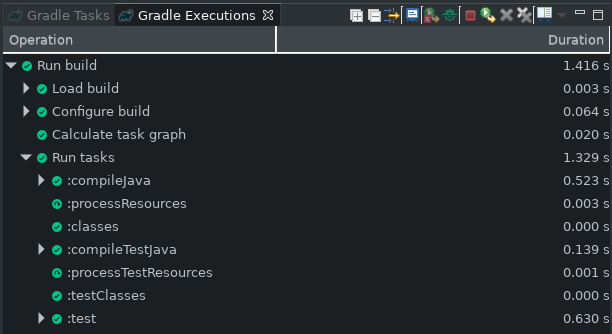
\includegraphics[width=1.0\linewidth, height=7cm]{3DependencyManagement/eclipsePlugin/gradleExecutionsView.png}
\end{subfigure}
\begin{subfigure}{0.5\textwidth}
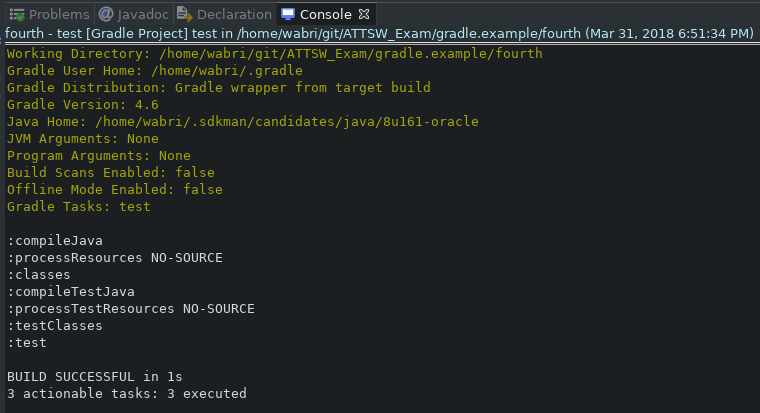
\includegraphics[width=1.1\linewidth, height=7cm]{3DependencyManagement/eclipsePlugin/consoleView.png}
\end{subfigure}
\end{figure}
Usando questi strumenti di Eclipse è possibile fare tutto ciò che prima veniva fatto da terminale.